\documentclass[1p]{elsarticle_modified}
%\bibliographystyle{elsarticle-num}

%\usepackage[colorlinks]{hyperref}
%\usepackage{abbrmath_seonhwa} %\Abb, \Ascr, \Acal ,\Abf, \Afrak
\usepackage{amsfonts}
\usepackage{amssymb}
\usepackage{amsmath}
\usepackage{amsthm}
\usepackage{scalefnt}
\usepackage{amsbsy}
\usepackage{kotex}
\usepackage{caption}
\usepackage{subfig}
\usepackage{color}
\usepackage{graphicx}
\usepackage{xcolor} %% white, black, red, green, blue, cyan, magenta, yellow
\usepackage{float}
\usepackage{setspace}
\usepackage{hyperref}

\usepackage{tikz}
\usetikzlibrary{arrows}

\usepackage{multirow}
\usepackage{array} % fixed length table
\usepackage{hhline}

%%%%%%%%%%%%%%%%%%%%%
\makeatletter
\renewcommand*\env@matrix[1][\arraystretch]{%
	\edef\arraystretch{#1}%
	\hskip -\arraycolsep
	\let\@ifnextchar\new@ifnextchar
	\array{*\c@MaxMatrixCols c}}
\makeatother %https://tex.stackexchange.com/questions/14071/how-can-i-increase-the-line-spacing-in-a-matrix
%%%%%%%%%%%%%%%

\usepackage[normalem]{ulem}

\newcommand{\msout}[1]{\ifmmode\text{\sout{\ensuremath{#1}}}\else\sout{#1}\fi}
%SOURCE: \msout is \stkout macro in https://tex.stackexchange.com/questions/20609/strikeout-in-math-mode

\newcommand{\cancel}[1]{
	\ifmmode
	{\color{red}\msout{#1}}
	\else
	{\color{red}\sout{#1}}
	\fi
}

\newcommand{\add}[1]{
	{\color{blue}\uwave{#1}}
}

\newcommand{\replace}[2]{
	\ifmmode
	{\color{red}\msout{#1}}{\color{blue}\uwave{#2}}
	\else
	{\color{red}\sout{#1}}{\color{blue}\uwave{#2}}
	\fi
}

\newcommand{\Sol}{\mathcal{S}} %segment
\newcommand{\D}{D} %diagram
\newcommand{\A}{\mathcal{A}} %arc


%%%%%%%%%%%%%%%%%%%%%%%%%%%%%5 test

\def\sl{\operatorname{\textup{SL}}(2,\Cbb)}
\def\psl{\operatorname{\textup{PSL}}(2,\Cbb)}
\def\quan{\mkern 1mu \triangleright \mkern 1mu}

\theoremstyle{definition}
\newtheorem{thm}{Theorem}[section]
\newtheorem{prop}[thm]{Proposition}
\newtheorem{lem}[thm]{Lemma}
\newtheorem{ques}[thm]{Question}
\newtheorem{cor}[thm]{Corollary}
\newtheorem{defn}[thm]{Definition}
\newtheorem{exam}[thm]{Example}
\newtheorem{rmk}[thm]{Remark}
\newtheorem{alg}[thm]{Algorithm}

\newcommand{\I}{\sqrt{-1}}
\begin{document}

%\begin{frontmatter}
%
%\title{Boundary parabolic representations of knots up to 8 crossings}
%
%%% Group authors per affiliation:
%\author{Yunhi Cho} 
%\address{Department of Mathematics, University of Seoul, Seoul, Korea}
%\ead{yhcho@uos.ac.kr}
%
%
%\author{Seonhwa Kim} %\fnref{s_kim}}
%\address{Center for Geometry and Physics, Institute for Basic Science, Pohang, 37673, Korea}
%\ead{ryeona17@ibs.re.kr}
%
%\author{Hyuk Kim}
%\address{Department of Mathematical Sciences, Seoul National University, Seoul 08826, Korea}
%\ead{hyukkim@snu.ac.kr}
%
%\author{Seokbeom Yoon}
%\address{Department of Mathematical Sciences, Seoul National University, Seoul, 08826,  Korea}
%\ead{sbyoon15@snu.ac.kr}
%
%\begin{abstract}
%We find all boundary parabolic representation of knots up to 8 crossings.
%
%\end{abstract}
%\begin{keyword}
%    \MSC[2010] 57M25 
%\end{keyword}
%
%\end{frontmatter}

%\linenumbers
%\tableofcontents
%
\newcommand\colored[1]{\textcolor{white}{\rule[-0.35ex]{0.8em}{1.4ex}}\kern-0.8em\color{red} #1}%
%\newcommand\colored[1]{\textcolor{white}{ #1}\kern-2.17ex	\textcolor{white}{ #1}\kern-1.81ex	\textcolor{white}{ #1}\kern-2.15ex\color{red}#1	}

{\Large $\underline{11n_{83}~(K11n_{83})}$}

\setlength{\tabcolsep}{10pt}
\renewcommand{\arraystretch}{1.6}
\vspace{1cm}\begin{tabular}{m{100pt}>{\centering\arraybackslash}m{274pt}}
\multirow{5}{120pt}{
	\centering
	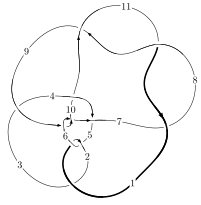
\includegraphics[width=112pt]{../../../GIT/diagram.site/Diagrams/png/699_11n_83.png}\\
\ \ \ A knot diagram\footnotemark}&
\allowdisplaybreaks
\textbf{Linearized knot diagam} \\
\cline{2-2}
 &
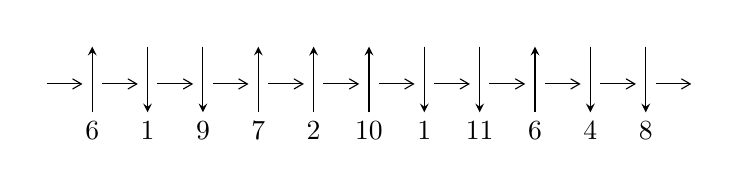
\begin{tikzpicture}[x=20pt, y=17pt]
	% nodes
	\node (C0) at (0, 0) {};
	\node (C1) at (1, 0) {};
	\node (C1U) at (1, +1) {};
	\node (C1D) at (1, -1) {6};

	\node (C2) at (2, 0) {};
	\node (C2U) at (2, +1) {};
	\node (C2D) at (2, -1) {1};

	\node (C3) at (3, 0) {};
	\node (C3U) at (3, +1) {};
	\node (C3D) at (3, -1) {9};

	\node (C4) at (4, 0) {};
	\node (C4U) at (4, +1) {};
	\node (C4D) at (4, -1) {7};

	\node (C5) at (5, 0) {};
	\node (C5U) at (5, +1) {};
	\node (C5D) at (5, -1) {2};

	\node (C6) at (6, 0) {};
	\node (C6U) at (6, +1) {};
	\node (C6D) at (6, -1) {10};

	\node (C7) at (7, 0) {};
	\node (C7U) at (7, +1) {};
	\node (C7D) at (7, -1) {1};

	\node (C8) at (8, 0) {};
	\node (C8U) at (8, +1) {};
	\node (C8D) at (8, -1) {11};

	\node (C9) at (9, 0) {};
	\node (C9U) at (9, +1) {};
	\node (C9D) at (9, -1) {6};

	\node (C10) at (10, 0) {};
	\node (C10U) at (10, +1) {};
	\node (C10D) at (10, -1) {4};

	\node (C11) at (11, 0) {};
	\node (C11U) at (11, +1) {};
	\node (C11D) at (11, -1) {8};
	\node (C12) at (12, 0) {};

	% arrows
	\draw[->,>={angle 60}]
	(C0) edge (C1) (C1) edge (C2) (C2) edge (C3) (C3) edge (C4) (C4) edge (C5) (C5) edge (C6) (C6) edge (C7) (C7) edge (C8) (C8) edge (C9) (C9) edge (C10) (C10) edge (C11) (C11) edge (C12) ;	\draw[->,>=stealth]
	(C1D) edge (C1U) (C2U) edge (C2D) (C3U) edge (C3D) (C4D) edge (C4U) (C5D) edge (C5U) (C6D) edge (C6U) (C7U) edge (C7D) (C8U) edge (C8D) (C9D) edge (C9U) (C10U) edge (C10D) (C11U) edge (C11D) ;
	\end{tikzpicture} \\
\hhline{~~} \\& 
\textbf{Solving Sequence} \\ \cline{2-2} 
 &
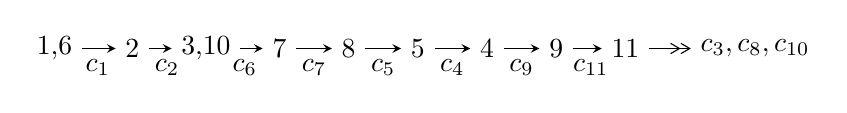
\begin{tikzpicture}[x=25pt, y=7pt]
	% node
	\node (A0) at (-1/8, 0) {1,6};
	\node (A1) at (1, 0) {2};
	\node (A2) at (33/16, 0) {3,10};
	\node (A3) at (25/8, 0) {7};
	\node (A4) at (33/8, 0) {8};
	\node (A5) at (41/8, 0) {5};
	\node (A6) at (49/8, 0) {4};
	\node (A7) at (57/8, 0) {9};
	\node (A8) at (65/8, 0) {11};
	\node (C1) at (1/2, -1) {$c_{1}$};
	\node (C2) at (3/2, -1) {$c_{2}$};
	\node (C3) at (21/8, -1) {$c_{6}$};
	\node (C4) at (29/8, -1) {$c_{7}$};
	\node (C5) at (37/8, -1) {$c_{5}$};
	\node (C6) at (45/8, -1) {$c_{4}$};
	\node (C7) at (53/8, -1) {$c_{9}$};
	\node (C8) at (61/8, -1) {$c_{11}$};
	\node (A9) at (10, 0) {$c_{3},c_{8},c_{10}$};

	% edge
	\draw[->,>=stealth]	
	(A0) edge (A1) (A1) edge (A2) (A2) edge (A3) (A3) edge (A4) (A4) edge (A5) (A5) edge (A6) (A6) edge (A7) (A7) edge (A8) ;
	\draw[->>,>={angle 60}]	
	(A8) edge (A9);
\end{tikzpicture} \\ 

\end{tabular} \\

\footnotetext{
The image of knot diagram is generated by the software ``\textbf{Draw programme}" developed by Andrew Bartholomew(\url{http://www.layer8.co.uk/maths/draw/index.htm\#Running-draw}), where we modified some parts for our purpose(\url{https://github.com/CATsTAILs/LinksPainter}).
}\phantom \\ \newline 
\centering \textbf{Ideals for irreducible components\footnotemark of $X_{\text{par}}$} 
 
\begin{align*}
I^u_{1}&=\langle 
-1.65693\times10^{21} u^{29}-1.25426\times10^{22} u^{28}+\cdots+7.78277\times10^{21} b-2.65124\times10^{22},\\
\phantom{I^u_{1}}&\phantom{= \langle  }-1.16811\times10^{22} u^{29}-8.79857\times10^{22} u^{28}+\cdots+2.33483\times10^{22} a-1.51866\times10^{23},\\
\phantom{I^u_{1}}&\phantom{= \langle  }u^{30}+8 u^{29}+\cdots+59 u+9\rangle \\
I^u_{2}&=\langle 
b^2-2 b u- u+1,\;a- u-1,\;u^2+u+1\rangle \\
I^u_{3}&=\langle 
b+u,\;a+u+1,\;u^2+u+1\rangle \\
\\
\end{align*}
\raggedright * 3 irreducible components of $\dim_{\mathbb{C}}=0$, with total 36 representations.\\
\footnotetext{All coefficients of polynomials are rational numbers. But the coefficients are sometimes approximated in decimal forms when there is not enough margin.}
\newpage
\renewcommand{\arraystretch}{1}
\centering \section*{I. $I^u_{1}= \langle -1.66\times10^{21} u^{29}-1.25\times10^{22} u^{28}+\cdots+7.78\times10^{21} b-2.65\times10^{22},\;-1.17\times10^{22} u^{29}-8.80\times10^{22} u^{28}+\cdots+2.33\times10^{22} a-1.52\times10^{23},\;u^{30}+8 u^{29}+\cdots+59 u+9 \rangle$}
\flushleft \textbf{(i) Arc colorings}\\
\begin{tabular}{m{7pt} m{180pt} m{7pt} m{180pt} }
\flushright $a_{1}=$&$\begin{pmatrix}1\\0\end{pmatrix}$ \\
\flushright $a_{6}=$&$\begin{pmatrix}0\\u\end{pmatrix}$ \\
\flushright $a_{2}=$&$\begin{pmatrix}1\\- u^2\end{pmatrix}$ \\
\flushright $a_{3}=$&$\begin{pmatrix}u^2+1\\- u^2\end{pmatrix}$ \\
\flushright $a_{10}=$&$\begin{pmatrix}0.500296 u^{29}+3.76840 u^{28}+\cdots+34.8145 u+6.50436\\0.212897 u^{29}+1.61159 u^{28}+\cdots+17.2043 u+3.40655\end{pmatrix}$ \\
\flushright $a_{7}=$&$\begin{pmatrix}-0.195327 u^{29}-1.50953 u^{28}+\cdots-27.9406 u-7.82719\\-0.200124 u^{29}-1.50933 u^{28}+\cdots-14.4262 u-3.01543\end{pmatrix}$ \\
\flushright $a_{8}=$&$\begin{pmatrix}0.00479750 u^{29}-0.000201005 u^{28}+\cdots-13.5144 u-4.81176\\-0.200124 u^{29}-1.50933 u^{28}+\cdots-14.4262 u-3.01543\end{pmatrix}$ \\
\flushright $a_{5}=$&$\begin{pmatrix}- u\\u^3+u\end{pmatrix}$ \\
\flushright $a_{4}=$&$\begin{pmatrix}0.582123 u^{29}+4.29047 u^{28}+\cdots+43.1171 u+10.9976\\0.243597 u^{29}+1.73550 u^{28}+\cdots+12.1493 u+1.59905\end{pmatrix}$ \\
\flushright $a_{9}=$&$\begin{pmatrix}0.500296 u^{29}+3.76840 u^{28}+\cdots+34.8145 u+6.50436\\0.275979 u^{29}+2.11887 u^{28}+\cdots+26.5057 u+5.51226\end{pmatrix}$ \\
\flushright $a_{11}=$&$\begin{pmatrix}-0.378505 u^{29}-2.81515 u^{28}+\cdots-27.1883 u-5.12752\\0.163272 u^{29}+1.28132 u^{28}+\cdots+17.0522 u+4.24326\end{pmatrix}$\\ \flushright $a_{11}=$&$\begin{pmatrix}-0.378505 u^{29}-2.81515 u^{28}+\cdots-27.1883 u-5.12752\\0.163272 u^{29}+1.28132 u^{28}+\cdots+17.0522 u+4.24326\end{pmatrix}$\\&\end{tabular}
\flushleft \textbf{(ii) Obstruction class $= -1$}\\~\\
\flushleft \textbf{(iii) Cusp Shapes $= \frac{1349639825927485091569}{7782769931873059073724} u^{29}+\frac{9179424603349810678583}{7782769931873059073724} u^{28}+\cdots+\frac{153279025524269859187337}{7782769931873059073724} u+\frac{5608854558132017698152}{648564160989421589477}$}\\~\\
\newpage\renewcommand{\arraystretch}{1}
\flushleft \textbf{(iv) u-Polynomials at the component}\newline \\
\begin{tabular}{m{50pt}|m{274pt}}
Crossings & \hspace{64pt}u-Polynomials at each crossing \\
\hline $$\begin{aligned}c_{1},c_{5}\end{aligned}$$&$\begin{aligned}
&u^{30}-8 u^{29}+\cdots-59 u+9
\end{aligned}$\\
\hline $$\begin{aligned}c_{2}\end{aligned}$$&$\begin{aligned}
&u^{30}+32 u^{29}+\cdots+47 u+81
\end{aligned}$\\
\hline $$\begin{aligned}c_{3}\end{aligned}$$&$\begin{aligned}
&u^{30}-8 u^{28}+\cdots-3557 u+451
\end{aligned}$\\
\hline $$\begin{aligned}c_{4}\end{aligned}$$&$\begin{aligned}
&u^{30}+4 u^{29}+\cdots-295 u+1601
\end{aligned}$\\
\hline $$\begin{aligned}c_{6},c_{9}\end{aligned}$$&$\begin{aligned}
&u^{30}-3 u^{29}+\cdots+4 u+3
\end{aligned}$\\
\hline $$\begin{aligned}c_{7},c_{8},c_{11}\end{aligned}$$&$\begin{aligned}
&u^{30}- u^{29}+\cdots-16 u+4
\end{aligned}$\\
\hline $$\begin{aligned}c_{10}\end{aligned}$$&$\begin{aligned}
&u^{30}+2 u^{29}+\cdots- u+3
\end{aligned}$\\
\hline
\end{tabular}\\~\\
\newpage\renewcommand{\arraystretch}{1}
\flushleft \textbf{(v) Riley Polynomials at the component}\newline \\
\begin{tabular}{m{50pt}|m{274pt}}
Crossings & \hspace{64pt}Riley Polynomials at each crossing \\
\hline $$\begin{aligned}c_{1},c_{5}\end{aligned}$$&$\begin{aligned}
&y^{30}+32 y^{29}+\cdots+47 y+81
\end{aligned}$\\
\hline $$\begin{aligned}c_{2}\end{aligned}$$&$\begin{aligned}
&y^{30}-64 y^{29}+\cdots-221233 y+6561
\end{aligned}$\\
\hline $$\begin{aligned}c_{3}\end{aligned}$$&$\begin{aligned}
&y^{30}-16 y^{29}+\cdots-5277497 y+203401
\end{aligned}$\\
\hline $$\begin{aligned}c_{4}\end{aligned}$$&$\begin{aligned}
&y^{30}+24 y^{29}+\cdots+28807823 y+2563201
\end{aligned}$\\
\hline $$\begin{aligned}c_{6},c_{9}\end{aligned}$$&$\begin{aligned}
&y^{30}-9 y^{29}+\cdots-58 y+9
\end{aligned}$\\
\hline $$\begin{aligned}c_{7},c_{8},c_{11}\end{aligned}$$&$\begin{aligned}
&y^{30}+25 y^{29}+\cdots-32 y+16
\end{aligned}$\\
\hline $$\begin{aligned}c_{10}\end{aligned}$$&$\begin{aligned}
&y^{30}+8 y^{29}+\cdots+59 y+9
\end{aligned}$\\
\hline
\end{tabular}\\~\\
\newpage\flushleft \textbf{(vi) Complex Volumes and Cusp Shapes}
$$\begin{array}{c|c|c}  
\text{Solutions to }I^u_{1}& \I (\text{vol} + \sqrt{-1}CS) & \text{Cusp shape}\\
 \hline 
\begin{aligned}
u &= -0.289006 + 0.960575 I \\
a &= \phantom{-}0.341844 + 0.310737 I \\
b &= \phantom{-}0.004028 - 1.301360 I\end{aligned}
 & \phantom{-}4.98680 - 2.32242 I & -0.98983 + 4.15024 I \\ \hline\begin{aligned}
u &= -0.289006 - 0.960575 I \\
a &= \phantom{-}0.341844 - 0.310737 I \\
b &= \phantom{-}0.004028 + 1.301360 I\end{aligned}
 & \phantom{-}4.98680 + 2.32242 I & -0.98983 - 4.15024 I \\ \hline\begin{aligned}
u &= -0.827863 + 0.788133 I \\
a &= \phantom{-}0.610296 + 0.163041 I \\
b &= -0.907811 + 0.765680 I\end{aligned}
 & \phantom{-}0.80409 - 2.85458 I & -2.92837 + 5.79821 I \\ \hline\begin{aligned}
u &= -0.827863 - 0.788133 I \\
a &= \phantom{-}0.610296 - 0.163041 I \\
b &= -0.907811 - 0.765680 I\end{aligned}
 & \phantom{-}0.80409 + 2.85458 I & -2.92837 - 5.79821 I \\ \hline\begin{aligned}
u &= -0.215656 + 1.206980 I \\
a &= \phantom{-}0.182869 + 1.070300 I \\
b &= -0.07834 + 1.70158 I\end{aligned}
 & \phantom{-}3.45780 - 2.70205 I & \phantom{-}2.31582 + 3.42763 I \\ \hline\begin{aligned}
u &= -0.215656 - 1.206980 I \\
a &= \phantom{-}0.182869 - 1.070300 I \\
b &= -0.07834 - 1.70158 I\end{aligned}
 & \phantom{-}3.45780 + 2.70205 I & \phantom{-}2.31582 - 3.42763 I \\ \hline\begin{aligned}
u &= -0.956886 + 0.832908 I \\
a &= -0.124030 - 0.650953 I \\
b &= \phantom{-}1.108780 - 0.402600 I\end{aligned}
 & \phantom{-}4.02348 - 1.34734 I & \phantom{-}3.26214 + 0.58804 I \\ \hline\begin{aligned}
u &= -0.956886 - 0.832908 I \\
a &= -0.124030 + 0.650953 I \\
b &= \phantom{-}1.108780 + 0.402600 I\end{aligned}
 & \phantom{-}4.02348 + 1.34734 I & \phantom{-}3.26214 - 0.58804 I \\ \hline\begin{aligned}
u &= -1.194550 + 0.646359 I \\
a &= -0.806434 + 0.092426 I \\
b &= \phantom{-}1.66643 - 0.93121 I\end{aligned}
 & \phantom{-}4.62105 - 5.90679 I & \phantom{-}4.52831 + 6.63187 I \\ \hline\begin{aligned}
u &= -1.194550 - 0.646359 I \\
a &= -0.806434 - 0.092426 I \\
b &= \phantom{-}1.66643 + 0.93121 I\end{aligned}
 & \phantom{-}4.62105 + 5.90679 I & \phantom{-}4.52831 - 6.63187 I\\
 \hline 
 \end{array}$$\newpage$$\begin{array}{c|c|c}  
\text{Solutions to }I^u_{1}& \I (\text{vol} + \sqrt{-1}CS) & \text{Cusp shape}\\
 \hline 
\begin{aligned}
u &= \phantom{-}0.29191 + 1.42887 I \\
a &= \phantom{-}0.744398 - 0.614810 I \\
b &= -1.13746 - 1.62619 I\end{aligned}
 & -3.80529 + 5.57168 I & -1.0000 - 2.74433 I \\ \hline\begin{aligned}
u &= \phantom{-}0.29191 - 1.42887 I \\
a &= \phantom{-}0.744398 + 0.614810 I \\
b &= -1.13746 + 1.62619 I\end{aligned}
 & -3.80529 - 5.57168 I & -1.0000 + 2.74433 I \\ \hline\begin{aligned}
u &= \phantom{-}0.534931 + 0.013556 I \\
a &= \phantom{-}1.31577 + 1.24844 I \\
b &= -0.939218 - 0.571832 I\end{aligned}
 & \phantom{-}0.93475 + 2.30280 I & -1.24616 - 3.74570 I \\ \hline\begin{aligned}
u &= \phantom{-}0.534931 - 0.013556 I \\
a &= \phantom{-}1.31577 - 1.24844 I \\
b &= -0.939218 + 0.571832 I\end{aligned}
 & \phantom{-}0.93475 - 2.30280 I & -1.24616 + 3.74570 I \\ \hline\begin{aligned}
u &= \phantom{-}0.131917 + 0.513534 I \\
a &= -1.123520 - 0.076835 I \\
b &= \phantom{-}0.192615 + 0.679919 I\end{aligned}
 & -1.028650 - 0.891272 I & -5.65753 + 3.58094 I \\ \hline\begin{aligned}
u &= \phantom{-}0.131917 - 0.513534 I \\
a &= -1.123520 + 0.076835 I \\
b &= \phantom{-}0.192615 - 0.679919 I\end{aligned}
 & -1.028650 + 0.891272 I & -5.65753 - 3.58094 I \\ \hline\begin{aligned}
u &= -0.288296 + 0.396727 I \\
a &= -1.58170 - 1.42670 I \\
b &= -0.0250531 - 0.0445070 I\end{aligned}
 & \phantom{-}1.85260 - 1.11432 I & \phantom{-}2.87293 - 2.42323 I \\ \hline\begin{aligned}
u &= -0.288296 - 0.396727 I \\
a &= -1.58170 + 1.42670 I \\
b &= -0.0250531 + 0.0445070 I\end{aligned}
 & \phantom{-}1.85260 + 1.11432 I & \phantom{-}2.87293 + 2.42323 I \\ \hline\begin{aligned}
u &= -0.473408 + 0.105538 I \\
a &= \phantom{-}2.08968 + 0.90137 I \\
b &= -0.08348 + 1.42196 I\end{aligned}
 & \phantom{-}7.52373 - 0.32119 I & \phantom{-}8.17779 - 0.83002 I \\ \hline\begin{aligned}
u &= -0.473408 - 0.105538 I \\
a &= \phantom{-}2.08968 - 0.90137 I \\
b &= -0.08348 - 1.42196 I\end{aligned}
 & \phantom{-}7.52373 + 0.32119 I & \phantom{-}8.17779 + 0.83002 I\\
 \hline 
 \end{array}$$\newpage$$\begin{array}{c|c|c}  
\text{Solutions to }I^u_{1}& \I (\text{vol} + \sqrt{-1}CS) & \text{Cusp shape}\\
 \hline 
\begin{aligned}
u &= \phantom{-}0.01716 + 1.58025 I \\
a &= -0.639515 - 0.509136 I \\
b &= -0.029559 - 0.549776 I\end{aligned}
 & -4.75687 - 1.39165 I & \phantom{-0.000000 } 0 \\ \hline\begin{aligned}
u &= \phantom{-}0.01716 - 1.58025 I \\
a &= -0.639515 + 0.509136 I \\
b &= -0.029559 + 0.549776 I\end{aligned}
 & -4.75687 + 1.39165 I & \phantom{-0.000000 } 0 \\ \hline\begin{aligned}
u &= \phantom{-}0.09265 + 1.59384 I \\
a &= -0.666239 + 0.534839 I \\
b &= \phantom{-}0.455313 + 1.306320 I\end{aligned}
 & -8.24005 + 0.28940 I & \phantom{-0.000000 } 0 \\ \hline\begin{aligned}
u &= \phantom{-}0.09265 - 1.59384 I \\
a &= -0.666239 - 0.534839 I \\
b &= \phantom{-}0.455313 - 1.306320 I\end{aligned}
 & -8.24005 - 0.28940 I & \phantom{-0.000000 } 0 \\ \hline\begin{aligned}
u &= -0.17358 + 1.65624 I \\
a &= \phantom{-}0.598313 - 0.464993 I \\
b &= \phantom{-}0.030527 - 0.633530 I\end{aligned}
 & -4.52151 - 5.10629 I & \phantom{-0.000000 } 0 \\ \hline\begin{aligned}
u &= -0.17358 - 1.65624 I \\
a &= \phantom{-}0.598313 + 0.464993 I \\
b &= \phantom{-}0.030527 + 0.633530 I\end{aligned}
 & -4.52151 + 5.10629 I & \phantom{-0.000000 } 0 \\ \hline\begin{aligned}
u &= -0.22083 + 1.70141 I \\
a &= \phantom{-}0.625937 + 0.523734 I \\
b &= -0.49633 + 1.34756 I\end{aligned}
 & -7.86584 - 6.86749 I & \phantom{-0.000000 } 0 \\ \hline\begin{aligned}
u &= -0.22083 - 1.70141 I \\
a &= \phantom{-}0.625937 - 0.523734 I \\
b &= -0.49633 - 1.34756 I\end{aligned}
 & -7.86584 + 6.86749 I & \phantom{-0.000000 } 0 \\ \hline\begin{aligned}
u &= -0.42849 + 1.69223 I \\
a &= -0.623225 - 0.533526 I \\
b &= \phantom{-}1.23958 - 1.77796 I\end{aligned}
 & -2.92088 - 12.01220 I & \phantom{-0.000000 } 0 \\ \hline\begin{aligned}
u &= -0.42849 - 1.69223 I \\
a &= -0.623225 + 0.533526 I \\
b &= \phantom{-}1.23958 + 1.77796 I\end{aligned}
 & -2.92088 + 12.01220 I & \phantom{-0.000000 } 0\\
 \hline 
 \end{array}$$\newpage\newpage\renewcommand{\arraystretch}{1}
\centering \section*{II. $I^u_{2}= \langle b^2-2 b u- u+1,\;a- u-1,\;u^2+u+1 \rangle$}
\flushleft \textbf{(i) Arc colorings}\\
\begin{tabular}{m{7pt} m{180pt} m{7pt} m{180pt} }
\flushright $a_{1}=$&$\begin{pmatrix}1\\0\end{pmatrix}$ \\
\flushright $a_{6}=$&$\begin{pmatrix}0\\u\end{pmatrix}$ \\
\flushright $a_{2}=$&$\begin{pmatrix}1\\u+1\end{pmatrix}$ \\
\flushright $a_{3}=$&$\begin{pmatrix}- u\\u+1\end{pmatrix}$ \\
\flushright $a_{10}=$&$\begin{pmatrix}u+1\\b\end{pmatrix}$ \\
\flushright $a_{7}=$&$\begin{pmatrix}- u-1\\- b+u\end{pmatrix}$ \\
\flushright $a_{8}=$&$\begin{pmatrix}b-2 u-1\\- b+u\end{pmatrix}$ \\
\flushright $a_{5}=$&$\begin{pmatrix}- u\\u+1\end{pmatrix}$ \\
\flushright $a_{4}=$&$\begin{pmatrix}b-2 u+1\\- b u+2 u\end{pmatrix}$ \\
\flushright $a_{9}=$&$\begin{pmatrix}u+1\\b- u\end{pmatrix}$ \\
\flushright $a_{11}=$&$\begin{pmatrix}- b u- b-2\\2\end{pmatrix}$\\ \flushright $a_{11}=$&$\begin{pmatrix}- b u- b-2\\2\end{pmatrix}$\\&\end{tabular}
\flushleft \textbf{(ii) Obstruction class $= 1$}\\~\\
\flushleft \textbf{(iii) Cusp Shapes $= 4 u+8$}\\~\\
\newpage\renewcommand{\arraystretch}{1}
\flushleft \textbf{(iv) u-Polynomials at the component}\newline \\
\begin{tabular}{m{50pt}|m{274pt}}
Crossings & \hspace{64pt}u-Polynomials at each crossing \\
\hline $$\begin{aligned}c_{1},c_{2},c_{10}\end{aligned}$$&$\begin{aligned}
&(u^2+u+1)^2
\end{aligned}$\\
\hline $$\begin{aligned}c_{3}\end{aligned}$$&$\begin{aligned}
&u^4-2 u^3+u^2-6 u+9
\end{aligned}$\\
\hline $$\begin{aligned}c_{4}\end{aligned}$$&$\begin{aligned}
&u^4+2 u^3+u^2+6 u+9
\end{aligned}$\\
\hline $$\begin{aligned}c_{5}\end{aligned}$$&$\begin{aligned}
&(u^2- u+1)^2
\end{aligned}$\\
\hline $$\begin{aligned}c_{6}\end{aligned}$$&$\begin{aligned}
&(u-1)^4
\end{aligned}$\\
\hline $$\begin{aligned}c_{7},c_{8},c_{11}\end{aligned}$$&$\begin{aligned}
&(u^2+2)^2
\end{aligned}$\\
\hline $$\begin{aligned}c_{9}\end{aligned}$$&$\begin{aligned}
&(u+1)^4
\end{aligned}$\\
\hline
\end{tabular}\\~\\
\newpage\renewcommand{\arraystretch}{1}
\flushleft \textbf{(v) Riley Polynomials at the component}\newline \\
\begin{tabular}{m{50pt}|m{274pt}}
Crossings & \hspace{64pt}Riley Polynomials at each crossing \\
\hline $$\begin{aligned}c_{1},c_{2},c_{5}\\c_{10}\end{aligned}$$&$\begin{aligned}
&(y^2+y+1)^2
\end{aligned}$\\
\hline $$\begin{aligned}c_{3},c_{4}\end{aligned}$$&$\begin{aligned}
&y^4-2 y^3-5 y^2-18 y+81
\end{aligned}$\\
\hline $$\begin{aligned}c_{6},c_{9}\end{aligned}$$&$\begin{aligned}
&(y-1)^4
\end{aligned}$\\
\hline $$\begin{aligned}c_{7},c_{8},c_{11}\end{aligned}$$&$\begin{aligned}
&(y+2)^4
\end{aligned}$\\
\hline
\end{tabular}\\~\\
\newpage\flushleft \textbf{(vi) Complex Volumes and Cusp Shapes}
$$\begin{array}{c|c|c}  
\text{Solutions to }I^u_{2}& \I (\text{vol} + \sqrt{-1}CS) & \text{Cusp shape}\\
 \hline 
\begin{aligned}
u &= -0.500000 + 0.866025 I \\
a &= \phantom{-}0.500000 + 0.866025 I \\
b &= -0.500000 - 0.548188 I\end{aligned}
 & \phantom{-}6.57974 - 2.02988 I & \phantom{-}6.00000 + 3.46410 I \\ \hline\begin{aligned}
u &= -0.500000 + 0.866025 I \\
a &= \phantom{-}0.500000 + 0.866025 I \\
b &= -0.50000 + 2.28024 I\end{aligned}
 & \phantom{-}6.57974 - 2.02988 I & \phantom{-}6.00000 + 3.46410 I \\ \hline\begin{aligned}
u &= -0.500000 - 0.866025 I \\
a &= \phantom{-}0.500000 - 0.866025 I \\
b &= -0.500000 + 0.548188 I\end{aligned}
 & \phantom{-}6.57974 + 2.02988 I & \phantom{-}6.00000 - 3.46410 I \\ \hline\begin{aligned}
u &= -0.500000 - 0.866025 I \\
a &= \phantom{-}0.500000 - 0.866025 I \\
b &= -0.50000 - 2.28024 I\end{aligned}
 & \phantom{-}6.57974 + 2.02988 I & \phantom{-}6.00000 - 3.46410 I\\
 \hline 
 \end{array}$$\newpage\newpage\renewcommand{\arraystretch}{1}
\centering \section*{III. $I^u_{3}= \langle b+u,\;a+u+1,\;u^2+u+1 \rangle$}
\flushleft \textbf{(i) Arc colorings}\\
\begin{tabular}{m{7pt} m{180pt} m{7pt} m{180pt} }
\flushright $a_{1}=$&$\begin{pmatrix}1\\0\end{pmatrix}$ \\
\flushright $a_{6}=$&$\begin{pmatrix}0\\u\end{pmatrix}$ \\
\flushright $a_{2}=$&$\begin{pmatrix}1\\u+1\end{pmatrix}$ \\
\flushright $a_{3}=$&$\begin{pmatrix}- u\\u+1\end{pmatrix}$ \\
\flushright $a_{10}=$&$\begin{pmatrix}- u-1\\- u\end{pmatrix}$ \\
\flushright $a_{7}=$&$\begin{pmatrix}- u-1\\0\end{pmatrix}$ \\
\flushright $a_{8}=$&$\begin{pmatrix}- u-1\\0\end{pmatrix}$ \\
\flushright $a_{5}=$&$\begin{pmatrix}- u\\u+1\end{pmatrix}$ \\
\flushright $a_{4}=$&$\begin{pmatrix}- u+1\\u+1\end{pmatrix}$ \\
\flushright $a_{9}=$&$\begin{pmatrix}- u-1\\0\end{pmatrix}$ \\
\flushright $a_{11}=$&$\begin{pmatrix}1\\0\end{pmatrix}$\\ \flushright $a_{11}=$&$\begin{pmatrix}1\\0\end{pmatrix}$\\&\end{tabular}
\flushleft \textbf{(ii) Obstruction class $= 1$}\\~\\
\flushleft \textbf{(iii) Cusp Shapes $= 4 u+2$}\\~\\
\newpage\renewcommand{\arraystretch}{1}
\flushleft \textbf{(iv) u-Polynomials at the component}\newline \\
\begin{tabular}{m{50pt}|m{274pt}}
Crossings & \hspace{64pt}u-Polynomials at each crossing \\
\hline $$\begin{aligned}c_{1},c_{2},c_{3}\\c_{4}\end{aligned}$$&$\begin{aligned}
&u^2+u+1
\end{aligned}$\\
\hline $$\begin{aligned}c_{5},c_{10}\end{aligned}$$&$\begin{aligned}
&u^2- u+1
\end{aligned}$\\
\hline $$\begin{aligned}c_{6}\end{aligned}$$&$\begin{aligned}
&(u+1)^2
\end{aligned}$\\
\hline $$\begin{aligned}c_{7},c_{8},c_{11}\end{aligned}$$&$\begin{aligned}
&u^2
\end{aligned}$\\
\hline $$\begin{aligned}c_{9}\end{aligned}$$&$\begin{aligned}
&(u-1)^2
\end{aligned}$\\
\hline
\end{tabular}\\~\\
\newpage\renewcommand{\arraystretch}{1}
\flushleft \textbf{(v) Riley Polynomials at the component}\newline \\
\begin{tabular}{m{50pt}|m{274pt}}
Crossings & \hspace{64pt}Riley Polynomials at each crossing \\
\hline $$\begin{aligned}c_{1},c_{2},c_{3}\\c_{4},c_{5},c_{10}\end{aligned}$$&$\begin{aligned}
&y^2+y+1
\end{aligned}$\\
\hline $$\begin{aligned}c_{6},c_{9}\end{aligned}$$&$\begin{aligned}
&(y-1)^2
\end{aligned}$\\
\hline $$\begin{aligned}c_{7},c_{8},c_{11}\end{aligned}$$&$\begin{aligned}
&y^2
\end{aligned}$\\
\hline
\end{tabular}\\~\\
\newpage\flushleft \textbf{(vi) Complex Volumes and Cusp Shapes}
$$\begin{array}{c|c|c}  
\text{Solutions to }I^u_{3}& \I (\text{vol} + \sqrt{-1}CS) & \text{Cusp shape}\\
 \hline 
\begin{aligned}
u &= -0.500000 + 0.866025 I \\
a &= -0.500000 - 0.866025 I \\
b &= \phantom{-}0.500000 - 0.866025 I\end{aligned}
 & \phantom{-}1.64493 - 2.02988 I & \phantom{-0.000000 -}0. + 3.46410 I \\ \hline\begin{aligned}
u &= -0.500000 - 0.866025 I \\
a &= -0.500000 + 0.866025 I \\
b &= \phantom{-}0.500000 + 0.866025 I\end{aligned}
 & \phantom{-}1.64493 + 2.02988 I & \phantom{-0.000000 } 0. - 3.46410 I\\
 \hline 
 \end{array}$$\newpage
\newpage\renewcommand{\arraystretch}{1}
\centering \section*{ IV. u-Polynomials}
\begin{tabular}{m{50pt}|m{274pt}}
Crossings & \hspace{64pt}u-Polynomials at each crossing \\
\hline $$\begin{aligned}c_{1}\end{aligned}$$&$\begin{aligned}
&((u^2+u+1)^3)(u^{30}-8 u^{29}+\cdots-59 u+9)
\end{aligned}$\\
\hline $$\begin{aligned}c_{2}\end{aligned}$$&$\begin{aligned}
&((u^2+u+1)^3)(u^{30}+32 u^{29}+\cdots+47 u+81)
\end{aligned}$\\
\hline $$\begin{aligned}c_{3}\end{aligned}$$&$\begin{aligned}
&(u^2+u+1)(u^4-2 u^3+u^2-6 u+9)(u^{30}-8 u^{28}+\cdots-3557 u+451)
\end{aligned}$\\
\hline $$\begin{aligned}c_{4}\end{aligned}$$&$\begin{aligned}
&(u^2+u+1)(u^4+2 u^3+u^2+6 u+9)(u^{30}+4 u^{29}+\cdots-295 u+1601)
\end{aligned}$\\
\hline $$\begin{aligned}c_{5}\end{aligned}$$&$\begin{aligned}
&((u^2- u+1)^3)(u^{30}-8 u^{29}+\cdots-59 u+9)
\end{aligned}$\\
\hline $$\begin{aligned}c_{6}\end{aligned}$$&$\begin{aligned}
&((u-1)^4)(u+1)^2(u^{30}-3 u^{29}+\cdots+4 u+3)
\end{aligned}$\\
\hline $$\begin{aligned}c_{7},c_{8},c_{11}\end{aligned}$$&$\begin{aligned}
&u^2(u^2+2)^2(u^{30}- u^{29}+\cdots-16 u+4)
\end{aligned}$\\
\hline $$\begin{aligned}c_{9}\end{aligned}$$&$\begin{aligned}
&((u-1)^2)(u+1)^4(u^{30}-3 u^{29}+\cdots+4 u+3)
\end{aligned}$\\
\hline $$\begin{aligned}c_{10}\end{aligned}$$&$\begin{aligned}
&(u^2- u+1)(u^2+u+1)^2(u^{30}+2 u^{29}+\cdots- u+3)
\end{aligned}$\\
\hline
\end{tabular}\newpage\renewcommand{\arraystretch}{1}
\centering \section*{ V. Riley Polynomials}
\begin{tabular}{m{50pt}|m{274pt}}
Crossings & \hspace{64pt}Riley Polynomials at each crossing \\
\hline $$\begin{aligned}c_{1},c_{5}\end{aligned}$$&$\begin{aligned}
&((y^2+y+1)^3)(y^{30}+32 y^{29}+\cdots+47 y+81)
\end{aligned}$\\
\hline $$\begin{aligned}c_{2}\end{aligned}$$&$\begin{aligned}
&((y^2+y+1)^3)(y^{30}-64 y^{29}+\cdots-221233 y+6561)
\end{aligned}$\\
\hline $$\begin{aligned}c_{3}\end{aligned}$$&$\begin{aligned}
&(y^2+y+1)(y^4-2 y^3-5 y^2-18 y+81)\\
&\cdot(y^{30}-16 y^{29}+\cdots-5277497 y+203401)
\end{aligned}$\\
\hline $$\begin{aligned}c_{4}\end{aligned}$$&$\begin{aligned}
&(y^2+y+1)(y^4-2 y^3-5 y^2-18 y+81)\\
&\cdot(y^{30}+24 y^{29}+\cdots+28807823 y+2563201)
\end{aligned}$\\
\hline $$\begin{aligned}c_{6},c_{9}\end{aligned}$$&$\begin{aligned}
&((y-1)^6)(y^{30}-9 y^{29}+\cdots-58 y+9)
\end{aligned}$\\
\hline $$\begin{aligned}c_{7},c_{8},c_{11}\end{aligned}$$&$\begin{aligned}
&y^2(y+2)^4(y^{30}+25 y^{29}+\cdots-32 y+16)
\end{aligned}$\\
\hline $$\begin{aligned}c_{10}\end{aligned}$$&$\begin{aligned}
&((y^2+y+1)^3)(y^{30}+8 y^{29}+\cdots+59 y+9)
\end{aligned}$\\
\hline
\end{tabular}
\vskip 2pc
\end{document}